\section{Approach}
\label{sec:approach}

In this section we introduce some background knowledge on the topic model and its supervised variants. And later we propose our model utilizing the title information for question documents. 

% First we give a formal definition of the multi-label classification problem:

% Given a set of documents $\boldsymbol{D}$ of size $N$, each of which contains words $\boldsymbol{w}^{(d)}$ and labels $\boldsymbol{L}^{(d)}$,  we'd like to train a model which given a new document $d_{new}$ without labels could predict its appropriate labels.

\subsection{Supervised topic models}

At first we show how to adapt the unsupervised topic model to a supervised one which could establish the correspondence between topics and labels as proposed in \cite{ramage2009labeled}. Then we extend the model to incorporate information provided by document titles. 

We describe each document $d \in \{1,\cdots,D\}$ as a multinomial distribution $\theta^{(d)}$ on labels, and each label (same as the topic in conventional LDA's terms) $\beta \in \{1,\cdots,K\}$ as another multinomial distribution over words. Noted that $K$ in standard LDA is supposed to be provided by users, while here it's the number of unique labels in the document set. Then document generation process is as following:

\begin{enumerate}[1.]
\item For every label $k$, sample a multinomial label-word distribution $\beta_k \sim Dir(\cdot|\eta)$;
\item For each document $d$, sample a multinomial document-label distribution $\theta^{(d)} \sim Dir(\cdot|\alpha^{(d)})$, where entries in $\alpha^{(d)}$ are non-zero if and only if corresponding labels are observed;
\item In document $d$, do following steps to generate every word:
  \begin{enumerate}[(a)]
  \item sample a label $z$ for this word position from $\theta^{(d)}$;
  \item sample a word $w$ for this word position from $\beta_z$.
  \end{enumerate}
\end{enumerate}

\subsection{Incorporating question titles}
First we want to emphasize the functionality of a document's title, especially for those on Q\&A websites. Users on those sites tend to describe their problems succinctly yet informative, for example they would very likely tell how the problems behave, or in what software, or what the wrong message is. In addition, since the document set we used mainly focused on programming or mathematics, many question titles would contain crucial keywords (like some named entities), making the titles more valuable for making decisions.

\begin{figure}
\centering
% \begin{tikzpicture}
% \tikzstyle{main}=[circle, minimum size = 7mm, thick, draw =black!80, node distance = 8mm and 10mm]
% \tikzstyle{connect}=[-latex, thick]
% \tikzstyle{box}=[rectangle, draw=black!100]
%   \node[main] (sigma) [] {$\sigma$};
%   \node[main] (epsilon) [above=of sigma] {$\epsilon$};
%   \node[main] (alpha) [above=of epsilon] {$\alpha$};
%   \node[main] (theta) [right=of alpha] {$\theta$};
%   \node[main] (z) [right=of theta] {$z_w$};
%   \node[main, fill = black!10] (w) [right=of z] {$w$};
%   \node[main, fill = black!10] (lambda) [right=of epsilon] {$\Lambda$};
%   \node[main] (phi) [below=of lambda] {$\Phi$};
%   \node[main] (beta) [right=of w] {$\beta$};
%   \node[main] (eta) [below=of beta] {$\eta$};
%   \node[main, fill = black!10] (omega) [below=of z] {$\Omega$};
%   \node[main] (psi) [below=of omega] {$\Psi$};

%   \path (alpha) edge [connect] (theta)
%         (theta) edge [connect] (z)
%         (z) edge [connect] (w)
%         (beta) edge [connect] (w)
%         (epsilon) edge [connect] (theta)
%         (psi) edge [connect] (omega)
%         (omega) edge [connect] (theta)
%         (phi) edge [connect] (lambda)
%         (lambda) edge [connect] (theta)
%         (eta) edge [connect] (beta)
%         (sigma) edge [connect] (epsilon);
%   \node[rounded corners, inner sep=0mm, fit= (z) (w),label={[xshift=14mm, yshift=-11mm]\textbf{$N$}}] {};
%   \node[rounded corners, very thick, inner xsep=3.3mm, inner ysep=3.3mm, draw=black!100, fit= (z) (w)] {};  

%   \node[rounded corners, inner ysep=0mm, fit = (theta) (z) (w) (omega) (lambda), label={[xshift=24mm, yshift=-28mm]\textbf{$D$}}] {};] {};
%   \node[rounded corners, very thick, inner xsep=5mm, inner ysep=5mm, draw=black!100, fit = (theta) (z) (w) (omega) (lambda)] {};

%   \node[rounded corners, inner sep=0mm, fit= (beta),label={[xshift=5.1mm, yshift=-11mm]\textbf{$K$}}] {};
%   \node[rounded corners, very thick, inner xsep=3.3mm, inner ysep=3.3mm, draw=black!100, fit= (beta)] {};

%   \node[rounded corners, inner sep=0mm, fit= (epsilon),label={[xshift=5.1mm, yshift=-11mm]\textbf{$K$}}] {};
%   \node[rounded corners, very thick, inner xsep=3.3mm, inner ysep=3.3mm, draw=black!100, fit= (epsilon)] {};
% \end{tikzpicture}
\includegraphics[angle=0,origin=br, width=0.4\textwidth]{fig/qlda.eps}
\caption{Graphical model of Labeled Q-LDA: both observed labels $\Lambda$ and \emph{qinfo} $\Omega$ would influence the topic mixture $\theta$} \label{fig:qlda}
\end{figure}

In this paper, we proposed a model called Q-DLA (Question-LDA) based on L-LDA for documents having structures like \emph{title-body-labels}, in which we treated titles separately and model them in another way. Our model is depicted using graphical model notation in Figure \ref{fig:qlda}. In addition to original L-LDA's parameters we have random variables describing the title information and its corresponding relations to labels, thus the topic mixture for each document is dependent not only on the Dirichlet prior and observed labels but also on observed titles.

At first we believe the key information in document titles would be named entities (along with some useful nouns) which we would refer to as \emph{qinfo} hereafter in this paper. While all other parameters are the same as in L-LDA,  to better illustrate Figure \ref{fig:qlda}, we classify the random variables into 3 categories:

\begin{itemize}
\item \textbf{Variables of standard LDA}: $\alpha$, $\eta$ are the hyper-parameters of Dirichlet distributions as the prior for label-word distribution $\beta$ and document-label distribution $\theta$. $z$ is label assigned to every word and $w$ is the observed word;
\item \textbf{Variables describing labels}: $\Phi$ is the Bernoulli prior generating observed labels $\Lambda$;
\item \textbf{Variables describing \emph{qinfo}}: $\Omega$ denotes the observed \emph{qinfo} in the title sampled by the Bernoulli prior $\Psi$, and $\epsilon$ denotes the \emph{qinfo}-label distribution sampled by the prior $Dir(\cdot|\sigma)$. 
\end{itemize}

And the complete document generation process of our model is:

\begin{enumerate}[1.]
\item For every label $k$, sample label-word distribution $\beta_k \sim Dir(\cdot|\eta)$;
\item For every \emph{qinfo} $i$, sample \emph{qinfo}-label distribution $\epsilon_i \sim Dir(\cdot|\sigma)$;
\item For each document $d$, 
  \begin{enumerate}[(a)]
    \item sample document-label distribution $\theta^{\prime(d)} \sim Dir(\cdot|\alpha^{(d)})$, where entries in $\alpha^{(d)}$ are non-zero if and only if corresponding labels are observed;
    \item sample the \emph{qinfo} for this document $\Omega^{(d)} \sim Bernoulli(\cdot|\Psi)$, and denote them as $Q = \{i | \Omega^{(d)}_i = 1\}$;
    \item generate the final label mixture from the restricted label distribution and \emph{qinfo}-incurred label distribution \newline $\theta^{(d)} = \mathcal{F}(\theta^{\prime(d)}, \sum_{i=1}^{|Q|}{\epsilon_{Q_i}})$.  
  \end{enumerate}
\item In document $d$, do following steps to generate every word:
  \begin{enumerate}[(a)]
  \item sample a label $z$ for this word position from $\theta^{(d)}$;
  \item sample a word $w$ for this word position from $\beta_z$.
  \end{enumerate}
\end{enumerate}

In another words, while L-LDA tries to restrict the topic distribution using observed labels as the mask, knowledge about \emph{qinfo} $\Omega$ would provide more information to give every word in that document more freedom of assigning topics. The topic distribution $\theta^{(d)}$ is drawn like this:

\begin{align}
\label{equ:qlda1}
\text{step 1:} & & \boldsymbol{\theta}^{\prime(d)} = (\theta_{l_1},\cdots,\theta_{l_{M_d}})^T \sim Dir(L^{(d)} \times \boldsymbol{\alpha}) \\
\text{step 2:} & & \boldsymbol{\theta}^{(d)} = \mathcal{F}(\boldsymbol{\theta}^{\prime(d)},\sum_{i=1}^{|Q|}{\epsilon_{Q_i}}).
\label{equ:qlda2}
\end{align}

There are two points worth noticing: in Equation \ref{equ:qlda1}, $L^{(d)} \times \boldsymbol{\alpha}$ means the masked label distribution by observed labels, and in Equation \ref{equ:qlda2}, we did not specify the exact relations between the restricted $\theta^{\prime(d)}$ after step 1 from L-LDA and the accumulated distributions using observed \emph{qinfo} after renormalization, since a specific function of those two would make the model harder to solve using Gibbs sampling. To illustrate our intuition that \emph{qinfo} from titles would indeed improve the classification results, we only need to prove they are somehow relevant and the model parameters should reflect such relevance, and we did this when inferring the model parameters in Gibbs sampling.

To illustrate why our model works, we selected a question as the example. 

{\small 
    \begin{verbatim}
Title: Stemming text in java
Body : im searching for a possibility to stemm
strings in java. First I wanted to do it with 
lucene but all the examples I found in the web...
Label: lucene, stemming
    \end{verbatim}
}

After pre-calculating the \emph{qinfo}-label distribution of \emph{stemming}, label \emph{nlp} has a relatively high probability in its distribution. So in the question ``Stemming text in java'' with labels \emph{lucene} and \emph{stemming} shown above, instead of assigning only those two labels for each word and sampling iteratively, Q-LDA would also assign labels \emph{nlp} since in its title the \emph{qinfo} ``Stemming'' would contribute such label choice. In this way, the label-word distribution $\beta$ after inference could avoid being skewed by expanding the label choice for each word.

\subsection{Learning the model}
\label{subsec:learn}

The learning algorithm for the full model is difficult since the way $\Omega$ affects $\theta^{(d)}$ is intended to be indefinite, therefore we used a simplified model as the prototype, where the \emph{qinfo}-label distribution is observed. This can be achieved by simply counting the co-occurrences of \emph{qinfo} and labels, then normalize them to be the desired \emph{qinfo}-label distribution. 

Thus, in Gibbs sampling process, when determining target topics for a particular document to sample, besides ones specified by labels $\Lambda^{(d)}$, the model also samples topics added from $\sum_{i=1}^{|\Omega^{(d)}|}{\epsilon_{\Omega_i^{(d)}}}$. And we added those topics in a very intuitive way - first from the \emph{qinfo} we added the corresponding distributions together and renormalized them, then from this distribution we pick ones with highest probability. 

In this way, the topic distribution for every document is not only influenced by the labels but also titles. Furthermore, the pre-calculated \emph{qinfo}-label distributions in a certain degree could describe the dependencies among labels, thus integrating them in the model would probably improve the word-label assignment process.

\subsection{Multi-label classification}

We take the same strategy as L-LDA to do classification, that is when encountering new documents without labels we do the Gibbs sampling process like normal LDA instead of enumerating all possible label assignments and pick the one with maximum posterior probability. This method is reasonable since it does not only reduce the computational cost but also approximate the original way - sampling from all labels is similar to trying all label assignments.